

\section{Signal and background samples}

\begin{itemize}
	\item List of samples used for the studies
	\item brief details on how the signal samples has been generated and how data is stored now (miniaods)
\end{itemize}

\section{Event selection}

\begin{itemize}
	\item Different trigger choice $\rightarrow$  Lower tau pt selection;
	\item tau reconstruction commissioned down to 20 \gev (chosen variable for cuts optimization);
	\item MET cut removed (chosen variable for cuts optimization)
	\item Dijet delta eta cut removed (obsolete because strictly correlated to the $m_{jj}$ cut) 
	\item $m_{jj}$ cut removed (chosen variable for cuts optimization)
	\item \hadtau isolation requirement has still high impact on statistics
\end{itemize}

\section{Sensitivity and cross section limit studies}

\begin{itemize}
	\item Optimization of cuts to exclude signal at the lowest cross section;
	\item the reference study formula is $\dfrac{S}{\sqrt{B + (0.5 \cdot B)^{2}}} > 2$
	\item signal events can also be express as: $S = \epsilon ( Pt_{\tau} , m_{jj} ,  \met )\cdot \sigma \cdot L$
	\item The sensitivity study is done as function of 3 different variables: $\tau_{pt}$, MET and $m_{jj}$
	\item Background prediction in SR: two-fold ABCD method involving 2 different (Schematic rappresentation needed) correction factors
	\item LtoT conversion factor:
	\begin{itemize}
		\item $LtoT = A * B$;
		\item Events with at least 4 jets;
		\item A: (the matched tau is also tight isolated)/(at least one jet matched to a loose tau)
		\item B: (the matched tau is also tight isolated)/(at least one jet matched to a tau (no iso requirement))
		\item VBF conversion factor: same as before (Excluding removed cuts)
	\end{itemize}
		\item Min cross section for $m_{jj} < 200$ and $130 < \met < 150$;
		\item Need to show impact of the $Pt_{\tau}$ over the limit.
		\item Uncertanties over the conversion factors?
\end{itemize}

\begin{figure}[tbh!]
	\centering
	\begin{tabular}{cc}
		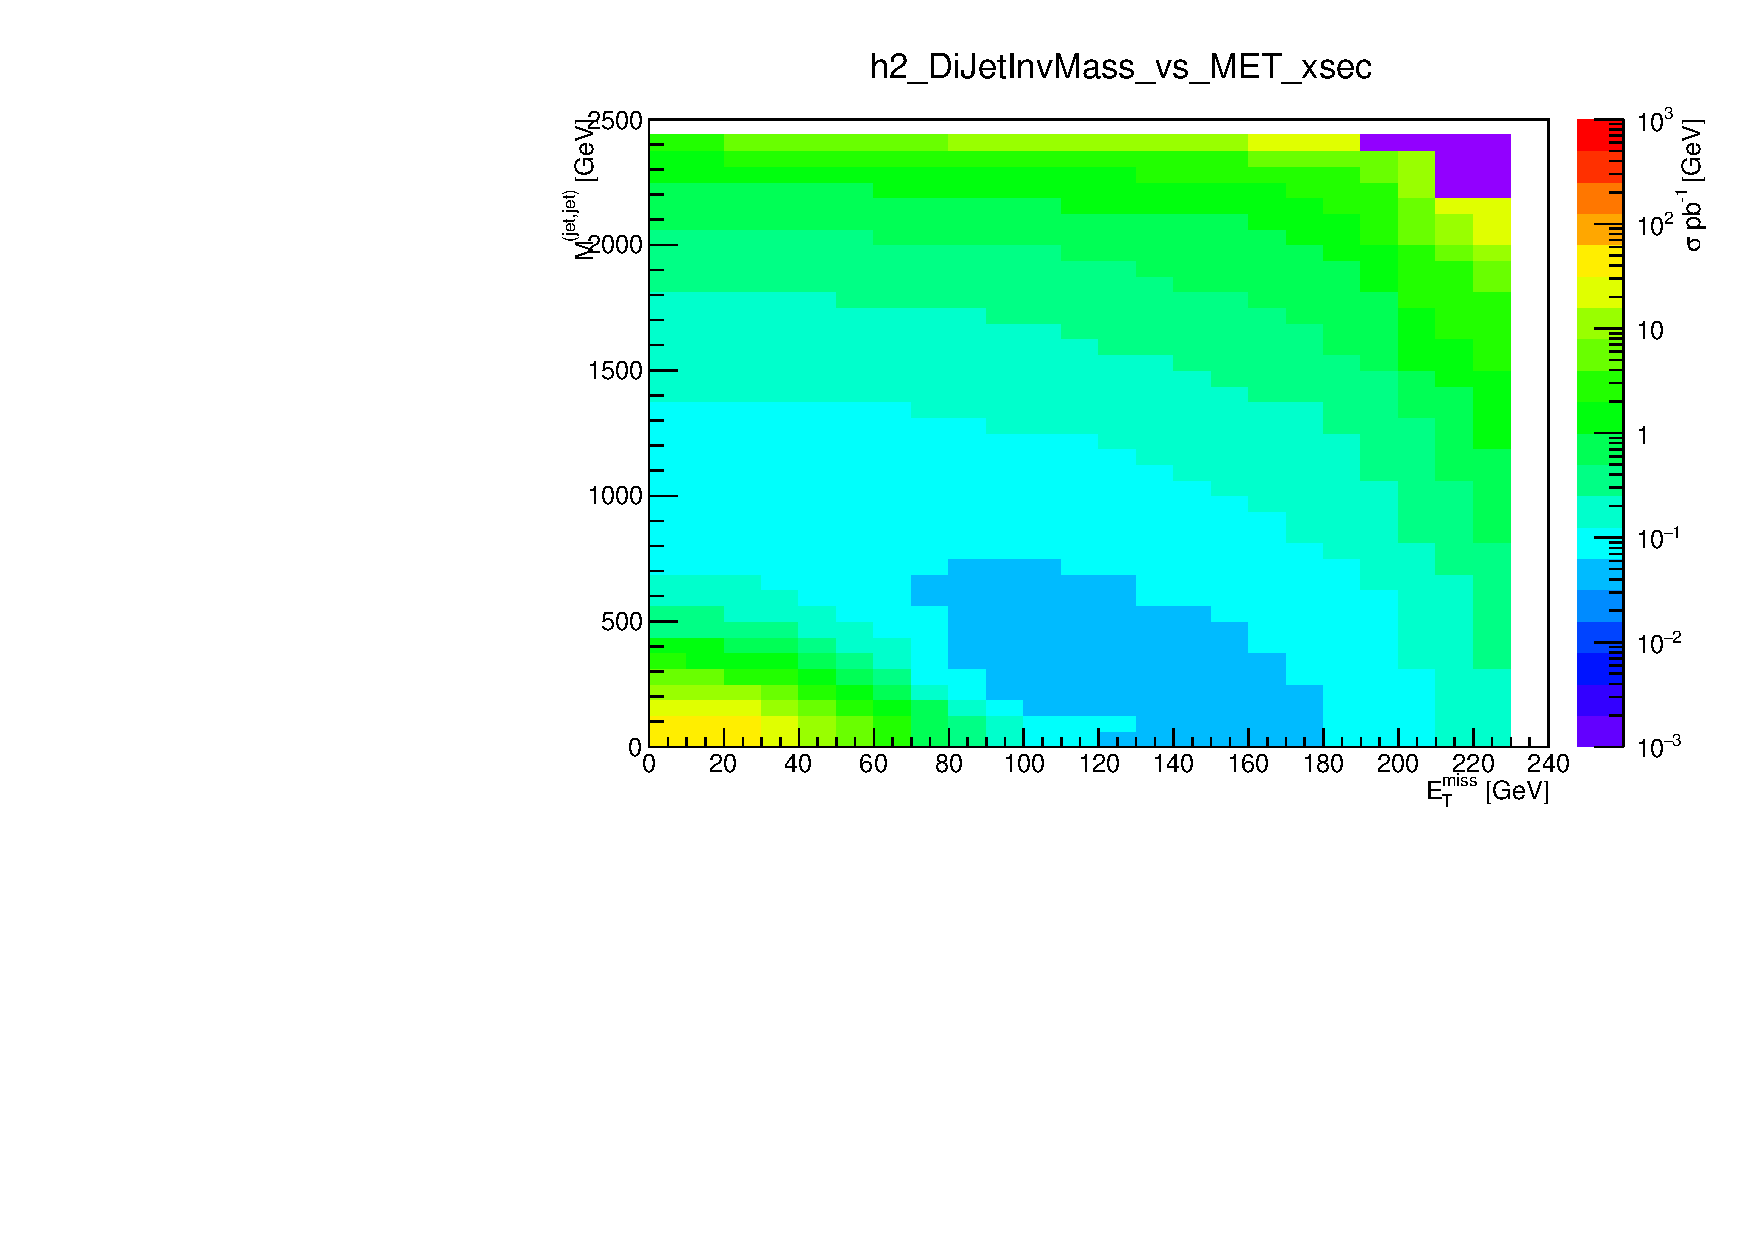
\includegraphics[width=0.48\textwidth]{analysis/pics/chi300_stau295_LSP0_taupt20.pdf}
		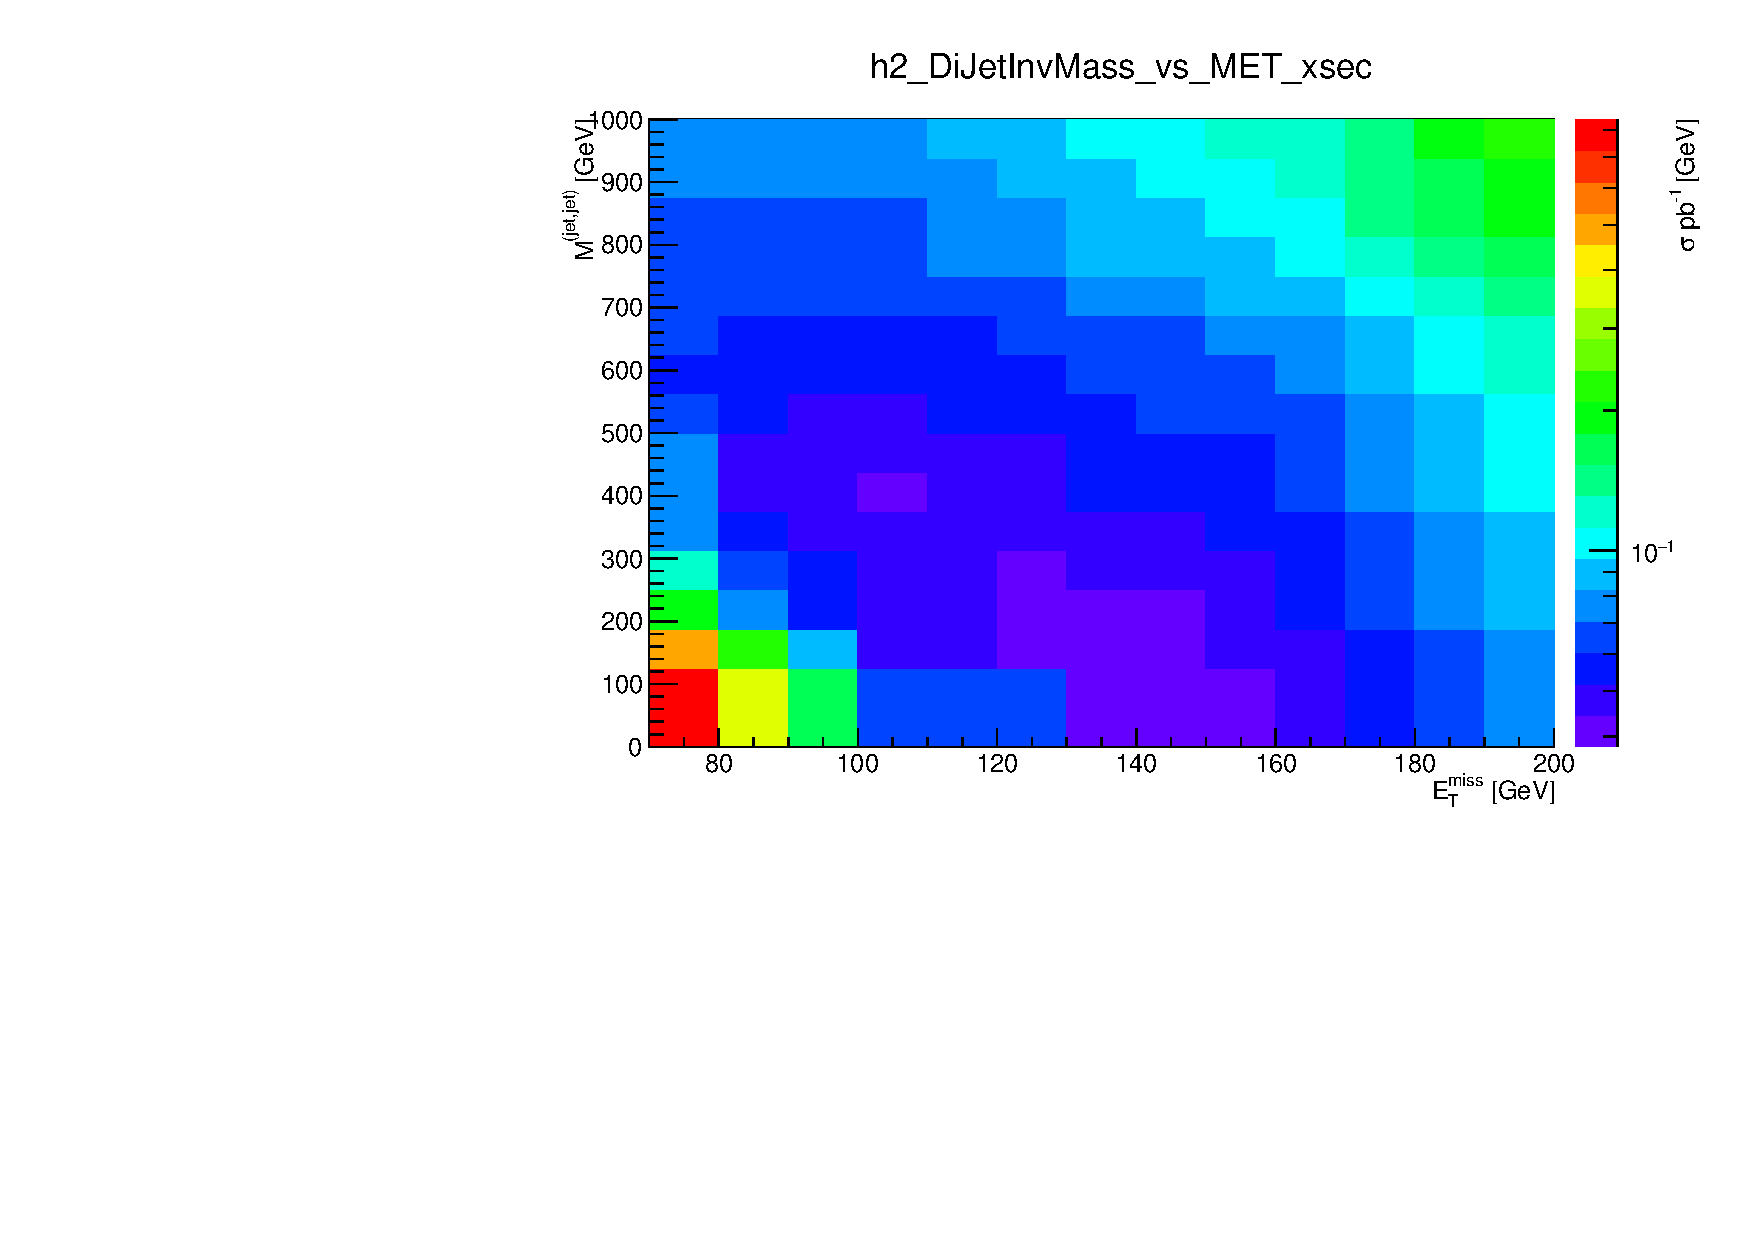
\includegraphics[width=0.48\textwidth]{analysis/pics/chi300_stau295_LSP0_taupt20_zoom.pdf} 		
	\end{tabular}
	\caption{chi300\_stau295\_LSP0\_taupt20}
\end{figure}

\begin{figure}[tbh!]
	\centering
	\begin{tabular}{cc}
		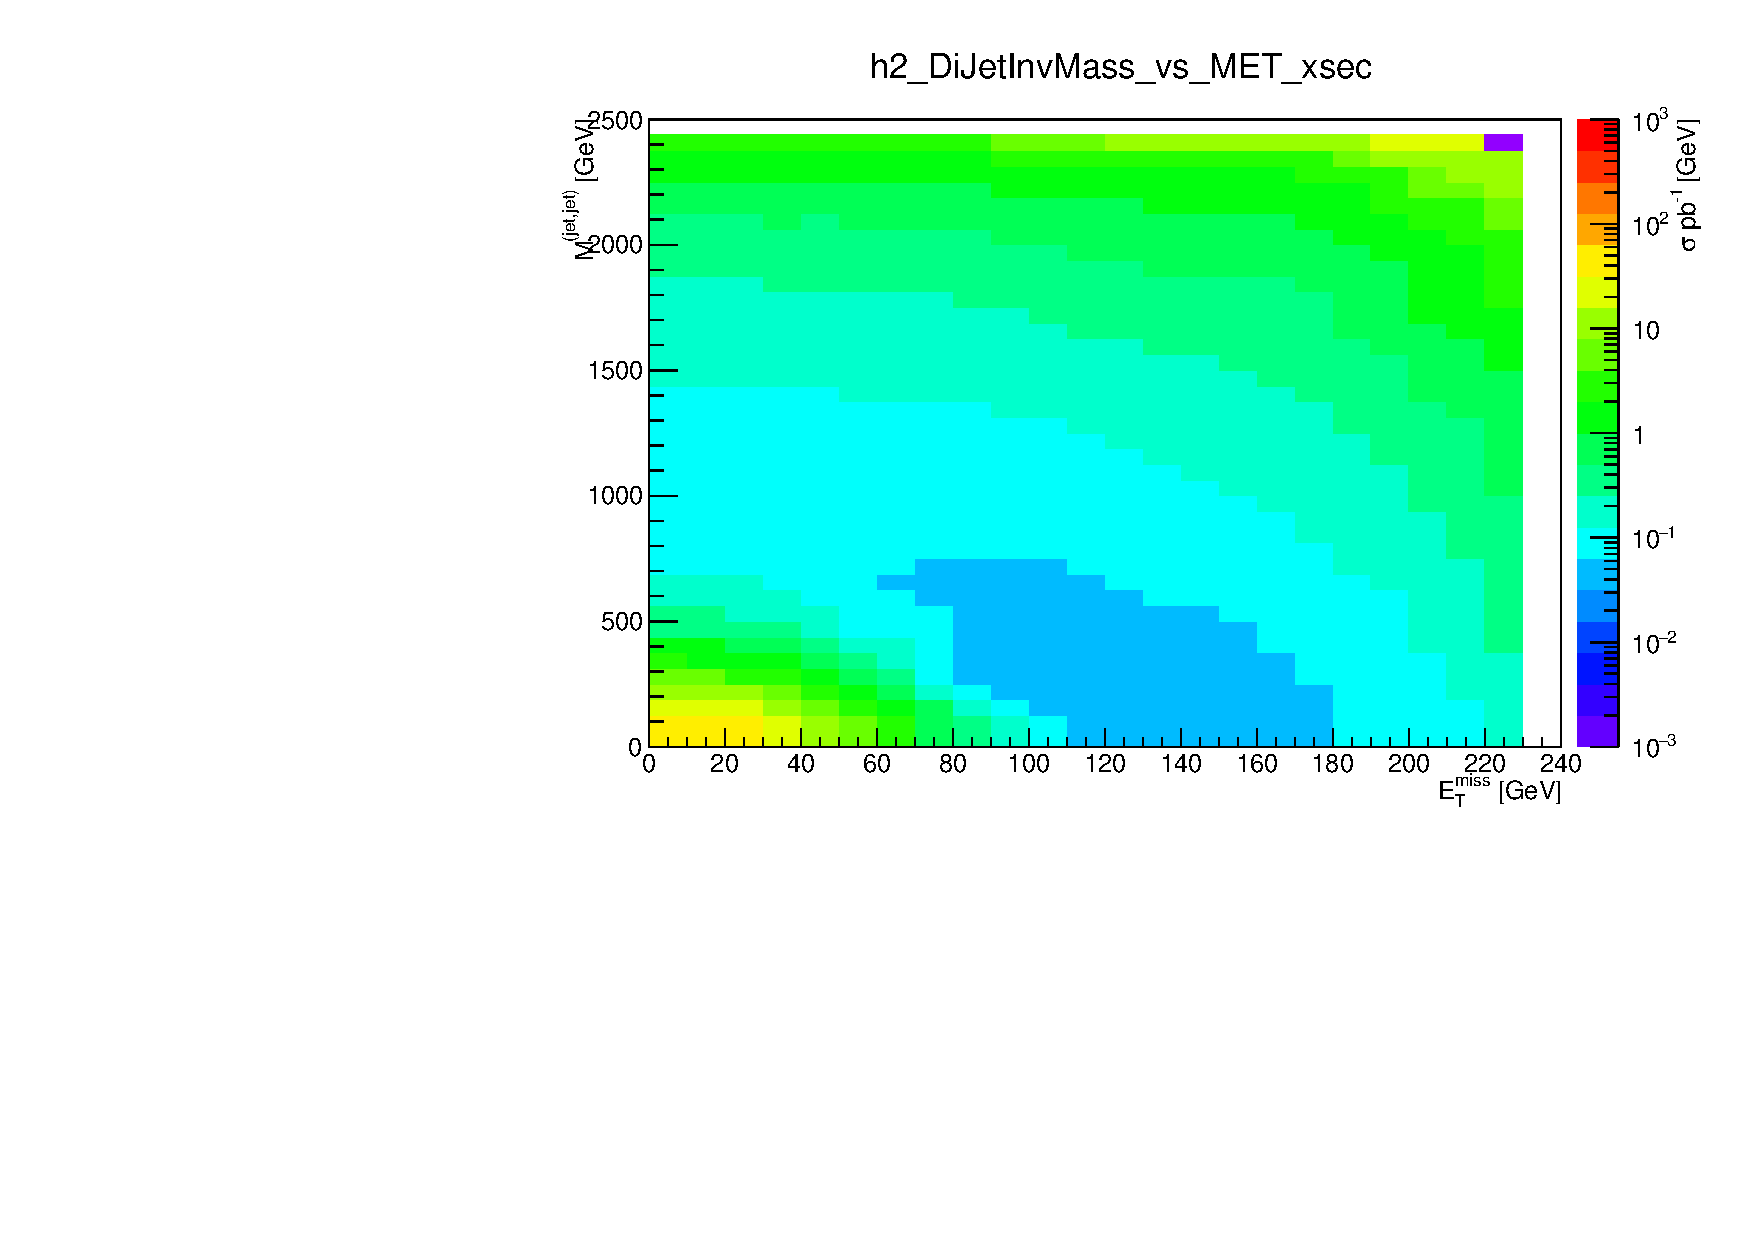
\includegraphics[width=0.48\textwidth]{analysis/pics/chi200_stau195_LSP0_taupt20.pdf}
		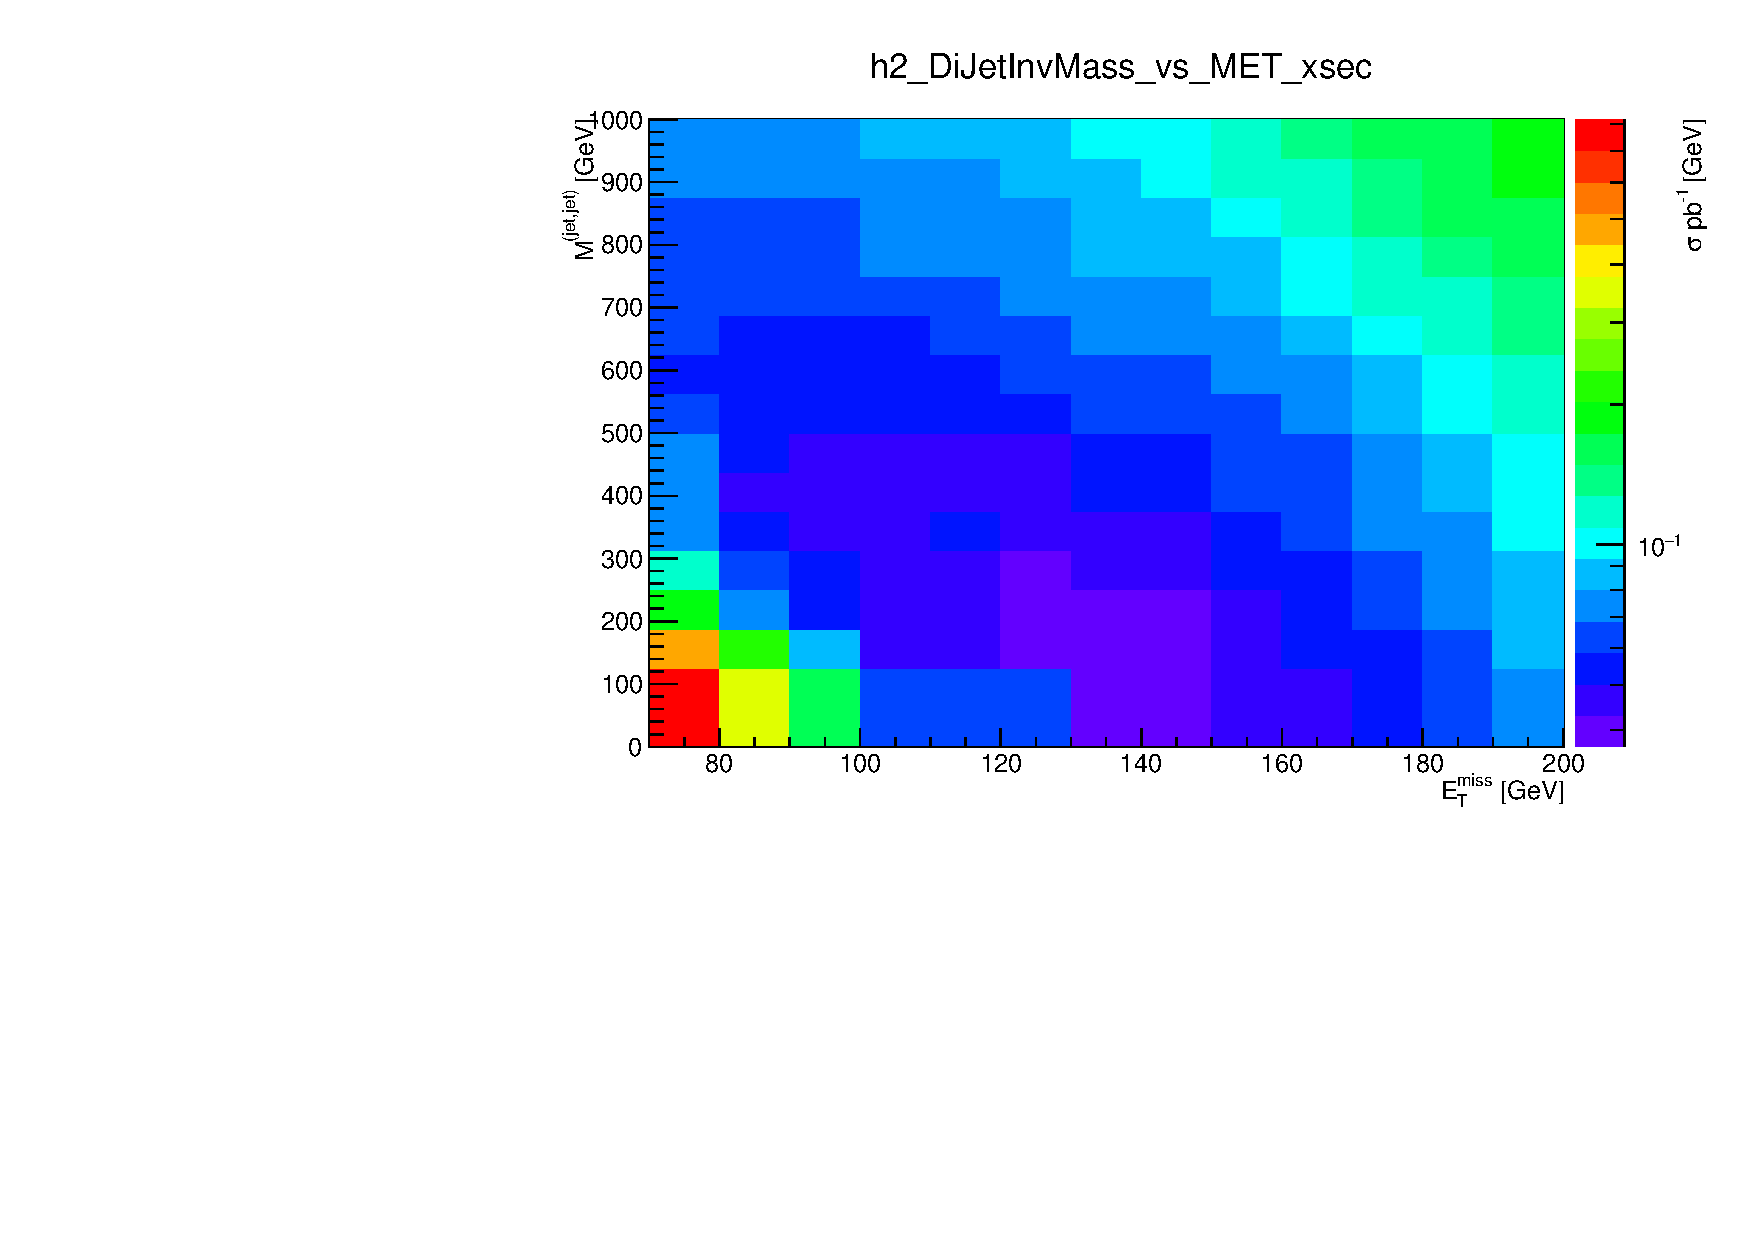
\includegraphics[width=0.48\textwidth]{analysis/pics/chi200_stau195_LSP0_taupt20_zoom.pdf} 		
	\end{tabular}
	\caption{chi200\_stau195\_LSP0\_taupt20}
\end{figure}

\begin{figure}[tbh!]
	\centering
	\begin{tabular}{cc}
		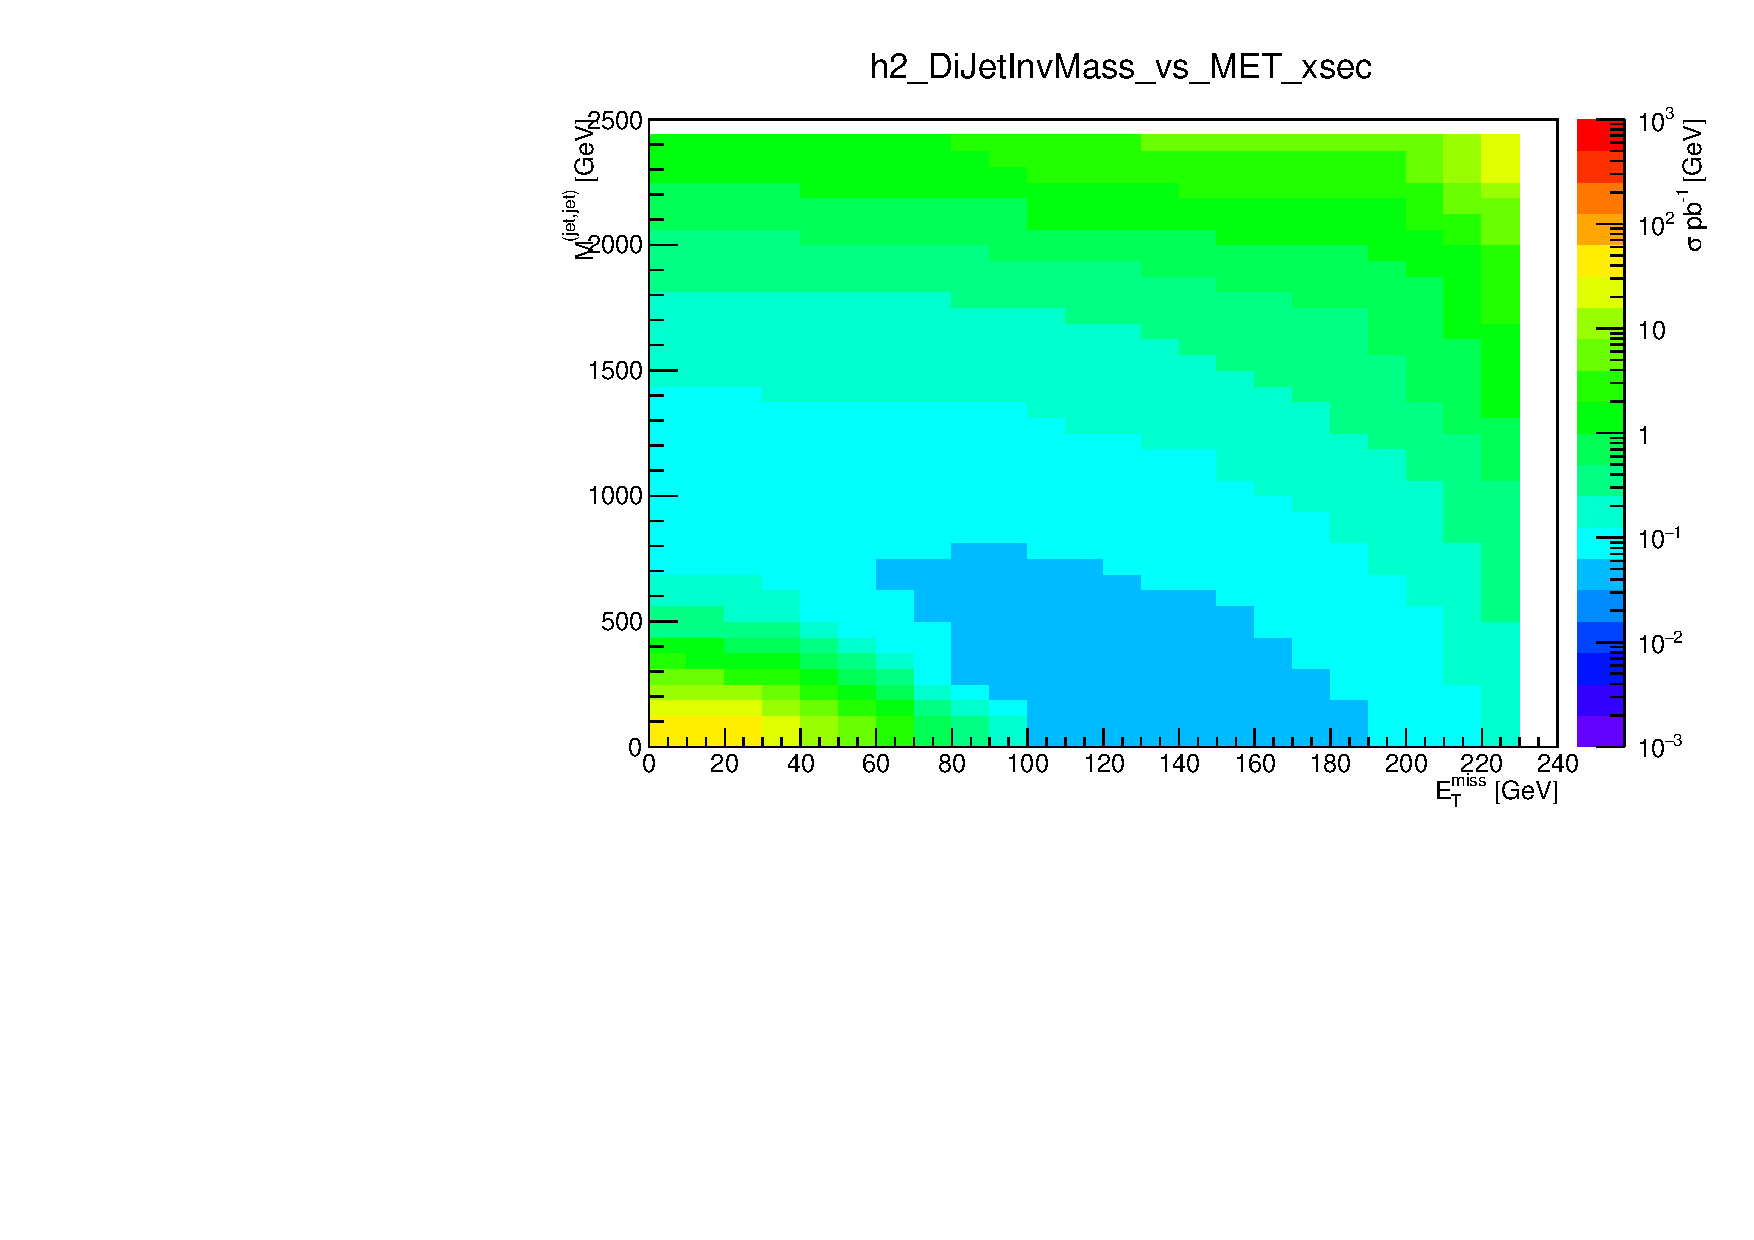
\includegraphics[width=0.48\textwidth]{analysis/pics/chi100_stau095_LSP0_taupt20.pdf}
		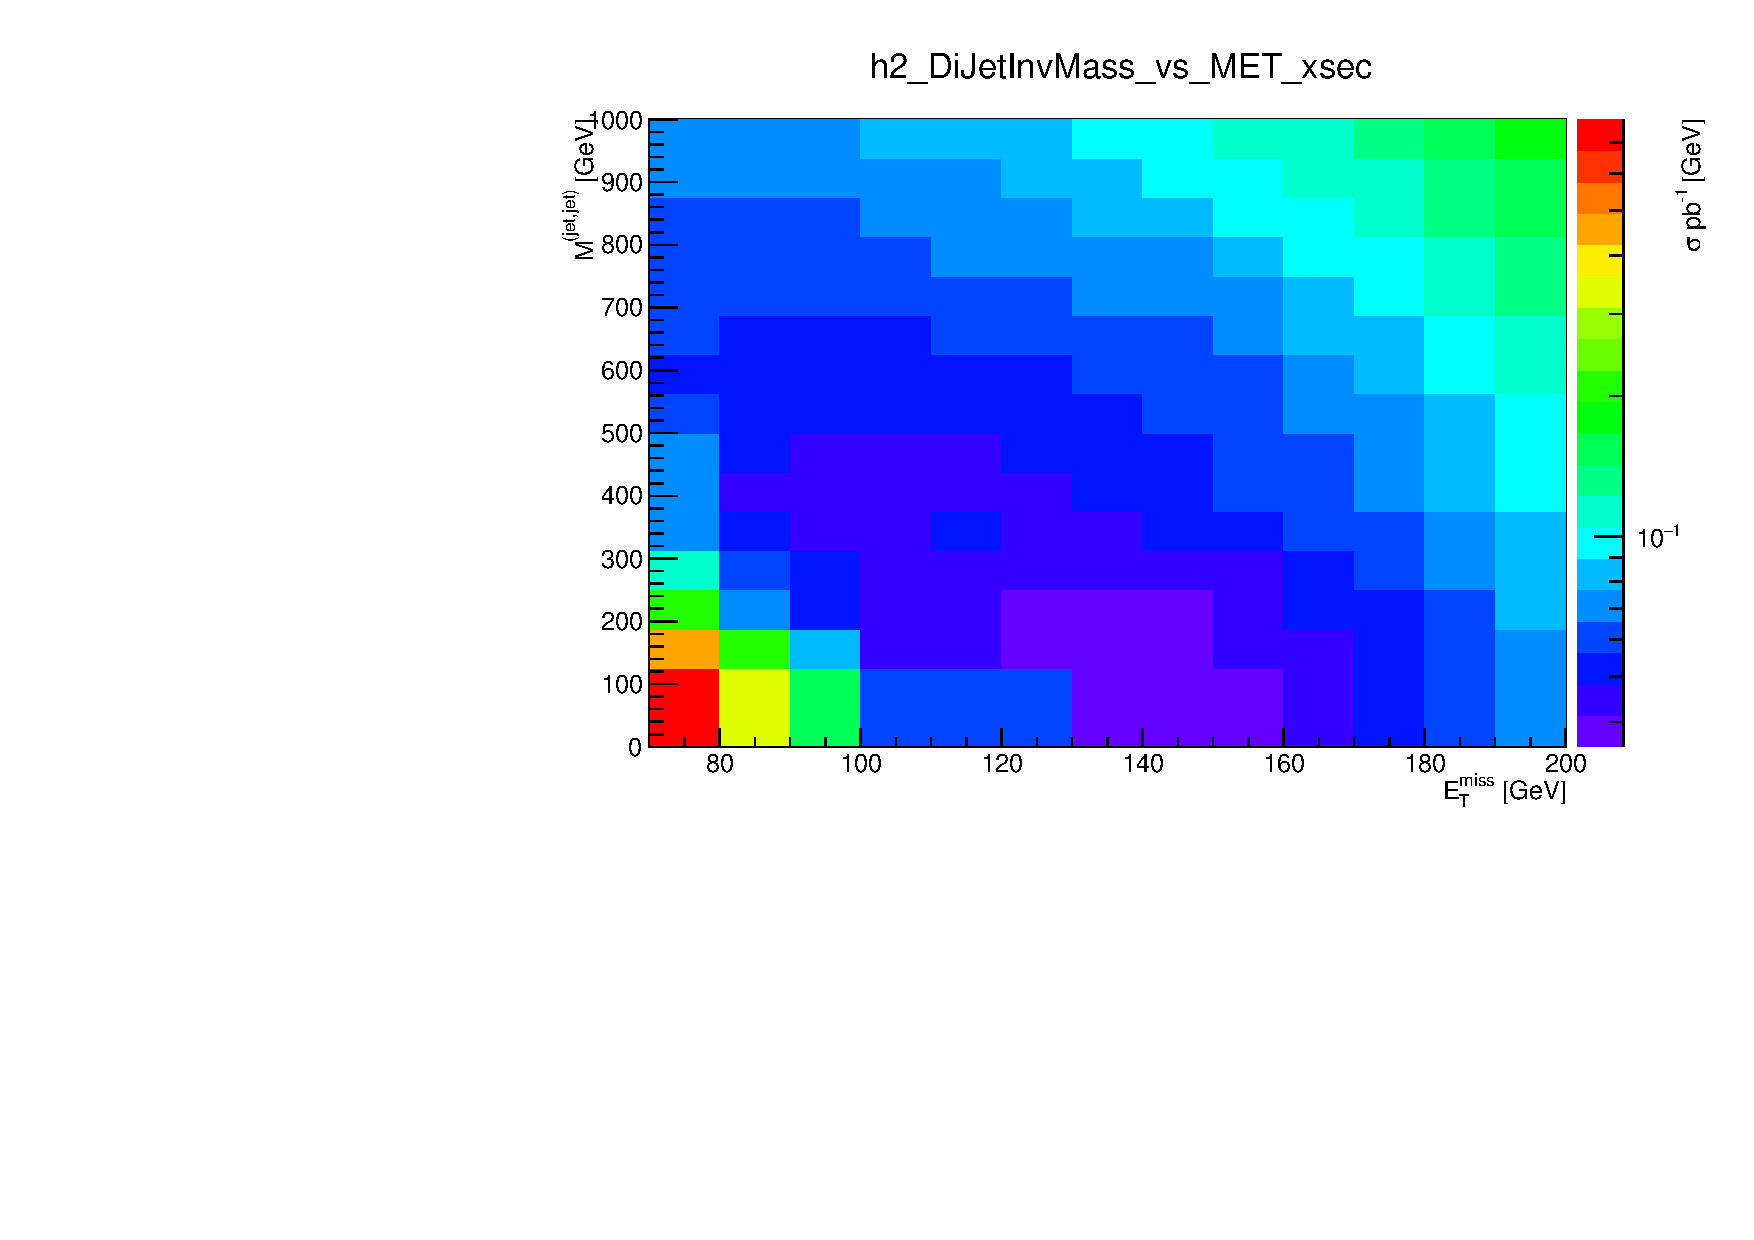
\includegraphics[width=0.48\textwidth]{analysis/pics/chi100_stau095_LSP0_taupt20_zoom.pdf} 		
	\end{tabular}
	\caption{chi100\_stau095\_LSP0\_taupt20}
\end{figure}
